\documentclass[12pt]{article}
\usepackage[left=1cm, right=1cm, top=2cm,bottom=1.5cm]{geometry} 

\usepackage[parfill]{parskip}
\usepackage[utf8]{inputenc}
\usepackage[T2A]{fontenc}
\usepackage[russian]{babel}
\usepackage{enumitem}
\usepackage[normalem]{ulem}
\usepackage{amsfonts, amsmath, amsthm, amssymb, mathtools,xcolor,accents}
\usepackage{blkarray}

\usepackage{tabularx}
\usepackage{hhline}

\usepackage{accents}
\usepackage{fancyhdr}
\pagestyle{fancy}
\renewcommand{\headrulewidth}{1.5pt}
\renewcommand{\footrulewidth}{1pt}

\usepackage{graphicx}
\usepackage[figurename=Рис.]{caption}
\usepackage{subcaption}
\usepackage{float}

%%Наименование папки откуда забирать изображения
\graphicspath{ {./images/} }

%%Изменение формата для ввода доказательства
\renewcommand{\proofname}{$\square$  \nopunct}
\renewcommand\qedsymbol{$\blacksquare$}

%%Изменение отступа на таблицах
\addto\captionsrussian{%
	\renewcommand{\proofname}{$\square$ \nopunct}%
}
%% Римские цифры
\newcommand{\RN}[1]{%
	\textup{\uppercase\expandafter{\romannumeral#1}}%
}

%% Для удобства записи
\newcommand{\MR}{\mathbb{R}}
\newcommand{\MC}{\mathbb{C}}
\newcommand{\MQ}{\mathbb{Q}}
\newcommand{\MN}{\mathbb{N}}
\newcommand{\MZ}{\mathbb{Z}}
\newcommand{\MTB}{\mathbb{T}}
\newcommand{\MTI}{\mathbb{I}}
\newcommand{\MI}{\mathrm{I}}
\newcommand{\MCI}{\mathcal{I}}
\newcommand{\MCR}{\mathcal{R}}
\newcommand{\MJ}{\mathrm{J}}
\newcommand{\MH}{\mathrm{H}}
\newcommand{\MT}{\mathrm{T}}
\newcommand{\MU}{\mathcal{U}}
\newcommand{\MV}{\mathcal{V}}
\newcommand{\MA}{\mathcal{A}}
\newcommand{\MB}{\mathcal{B}}
\newcommand{\MF}{\mathcal{F}}
\newcommand{\ME}{\mathcal{E}}
\newcommand{\MW}{\mathcal{W}}
\newcommand{\ML}{\mathcal{L}}
\newcommand{\MM}{\mathcal{M}}
\newcommand{\MP}{\mathcal{P}}
\newcommand{\VN}{\varnothing}
\newcommand{\VE}{\varepsilon}
\newcommand{\dx}{\, dx}
\newcommand{\dy}{\, dy}
\newcommand{\dz}{\, dz}
\newcommand{\dd}{\, d}


\theoremstyle{definition}
\newtheorem{defn}{Опр:}
\newtheorem{rem}{Rm:}
\newtheorem{prop}{Утв.}
\newtheorem{exrc}{Упр.}
\newtheorem{problem}{Задача}
\newtheorem{lemma}{Лемма}
\newtheorem{theorem}{Теорема}
\newtheorem{corollary}{Следствие}

\newenvironment{cusdefn}[1]
{\renewcommand\thedefn{#1}\defn}
{\enddefn}

\DeclareRobustCommand{\divby}{%
	\mathrel{\text{\vbox{\baselineskip.65ex\lineskiplimit0pt\hbox{.}\hbox{.}\hbox{.}}}}%
}
\DeclareRobustCommand{\ndivby}{\mkern-1mu\not\mathrel{\mkern4.5mu\divby}\mkern1mu}


%Короткий минус
\DeclareMathSymbol{\SMN}{\mathbin}{AMSa}{"39}
%Длинная шапка
\newcommand{\overbar}[1]{\mkern 1.5mu\overline{\mkern-1.5mu#1\mkern-1.5mu}\mkern 1.5mu}
%Функция знака
\DeclareMathOperator{\sgn}{sgn}

%Функция ранга
\DeclareMathOperator{\rk}{\text{rk}}
\DeclareMathOperator{\diam}{\text{diam}}


%Обозначение константы
\DeclareMathOperator{\const}{\text{const}}

\DeclareMathOperator{\codim}{\text{codim}}

\DeclareMathOperator*{\dsum}{\displaystyle\sum}
\newcommand{\ddsum}[2]{\displaystyle\sum\limits_{#1}^{#2}}
\newcommand{\ddssum}[2]{\displaystyle\smashoperator{\sum\limits_{#1}^{#2}}}
\newcommand{\ddlsum}[2]{\displaystyle\smashoperator[l]{\sum\limits_{#1}^{#2}}}
\newcommand{\ddrsum}[2]{\displaystyle\smashoperator[r]{\sum\limits_{#1}^{#2}}}

%Интеграл в большом формате
\DeclareMathOperator{\dint}{\displaystyle\int}
\newcommand{\ddint}[2]{\displaystyle\int\limits_{#1}^{#2}}
\newcommand{\ssum}[1]{\displaystyle \sum\limits_{n=1}^{\infty}{#1}_n}

\newcommand{\smallerrel}[1]{\mathrel{\mathpalette\smallerrelaux{#1}}}
\newcommand{\smallerrelaux}[2]{\raisebox{.1ex}{\scalebox{.75}{$#1#2$}}}

\newcommand{\smallin}{\smallerrel{\in}}
\newcommand{\smallnotin}{\smallerrel{\notin}}

\newcommand*{\medcap}{\mathbin{\scalebox{1.25}{\ensuremath{\cap}}}}%
\newcommand*{\medcup}{\mathbin{\scalebox{1.25}{\ensuremath{\cup}}}}%

\makeatletter
\newcommand{\vast}{\bBigg@{3.5}}
\newcommand{\Vast}{\bBigg@{5}}
\makeatother

%Промежуточное значение для sup\inf, поскольку они имеют разную высоту
\newcommand{\newsup}{\mathop{\smash{\mathrm{sup}}}}
\newcommand{\newinf}{\mathop{\mathrm{inf}\vphantom{\mathrm{sup}}}}

%Скалярное произведение
\newcommand{\inner}[2]{\left\langle #1, #2 \right\rangle }
\newcommand{\linsp}[1]{\left\langle #1 \right\rangle }
\newcommand{\linmer}[2]{\left\langle #1 \vert #2\right\rangle }

%Подпись символов снизу
\newcommand{\ubar}[1]{\underaccent{\bar}{#1}}

%%Шапка для букв сверху
\newcommand{\wte}[1]{\widetilde{#1}}
\newcommand{\wht}[1]{\widehat{#1}}
\newcommand{\ovl}[1]{\overline{#1}}
\newcommand{\unl}[1]{\underline{#1}}


%%Трансформация Фурье
\newcommand{\fourt}[1]{\mathcal{F}\left(#1\right)}
\newcommand{\ifourt}[1]{\mathcal{F}^{-1}\left(#1\right)}

%%Символ вектора
\newcommand{\vecm}[1]{\overrightarrow{#1\,}}

%%Пространстов матриц
\newcommand{\matsq}[1]{\operatorname{Mat}_{#1}}
\newcommand{\mat}[2]{\operatorname{Mat}_{#1, #2}}

%Оператор для действ и мнимых чисел
\DeclareMathOperator{\IM}{\operatorname{Im}}
\DeclareMathOperator{\RE}{\operatorname{Re}}
\DeclareMathOperator{\li}{\operatorname{li}}
\DeclareMathOperator{\GL}{\operatorname{GL}}
\DeclareMathOperator{\SL}{\operatorname{SL}}
\DeclareMathOperator{\Char}{\operatorname{char}}
\DeclareMathOperator\Arg{Arg}
\DeclareMathOperator\ord{ord}

%Оператор для образа
\DeclareMathOperator{\Ima}{Im}

%Делимость чисел
\newcommand{\modn}[3]{#1 \equiv #2 \; (\bmod \; #3)}
\newcommand{\nmodn}[3]{#1 \not\equiv #2 \; (\bmod \; #3)}

%%Взятие в скобки, модули и норму
\newcommand{\parfit}[1]{\left( #1 \right)}
\newcommand{\modfit}[1]{\left| #1 \right|}
\newcommand{\sqparfit}[1]{\left\{ #1 \right\}}
\newcommand{\normfit}[1]{\left\| #1 \right\|}

%%Функция для обозначения равномерной сходимости по множеству
\newcommand{\uconv}[1]{\overset{#1}{\rightrightarrows}}
\newcommand{\uconvm}[2]{\overset{#1}{\underset{#2}{\rightrightarrows}}}

%% Функция для добавления круга сверху множества
\newcommand{\Circ}[1]{\accentset{\circ}{#1}}

%% Жирное подчеркивание
\newcommand{\buline}[1]{\textbf{\uline{#1}}}

%%Функция для обозначения нижнего и верхнего интегралов
\def\upint{\mathchoice%
	{\mkern13mu\overline{\vphantom{\intop}\mkern7mu}\mkern-20mu}%
	{\mkern7mu\overline{\vphantom{\intop}\mkern7mu}\mkern-14mu}%
	{\mkern7mu\overline{\vphantom{\intop}\mkern7mu}\mkern-14mu}%
	{\mkern7mu\overline{\vphantom{\intop}\mkern7mu}\mkern-14mu}%
	\int}
\def\lowint{\mkern3mu\underline{\vphantom{\intop}\mkern7mu}\mkern-10mu\int}

%%След матрицы
\DeclareMathOperator*{\tr}{tr}

\DeclareMathOperator*{\symdif}{\bigtriangleup}

% Верхние\нижние пределы
\DeclareMathOperator*\lowlim{\underline{lim}}
\DeclareMathOperator*\uplim{\overline{lim}}

\makeatletter
\renewcommand*\env@matrix[1][*\c@MaxMatrixCols c]{%
	\hskip -\arraycolsep
	\let\@ifnextchar\new@ifnextchar
	\array{#1}}
\makeatother


%% Переопределение функции хи, чтобы выглядела более приятно
\makeatletter
\@ifdefinable\@latex@chi{\let\@latex@chi\chi}
\renewcommand*\chi{{\@latex@chi\smash[t]{\mathstrut}}} % want only bottom half of \mathstrut
\makeatletter

\setcounter{MaxMatrixCols}{20}

\begin{document}
\lhead{Аналитическая геометрия}
\chead{Пенской А.В.}
\rhead{Лекция - 4}
\section*{Векторная алгебра}

\begin{defn}
	\uwave{Направленный отрезок} - упорядоченная пара точек $[AB]$.
\end{defn}
\begin{defn}
	$[AB]$ и $[CD]$ \uwave{коллинеарны} (параллельны), если прямые $AB$ и $CD$ - параллельны или совпадают.
\end{defn}
\begin{defn}
	\uwave{Длиной направленного отрезка} называется длина соответствующего отрезка: $|[AB]| = |AB| \geq 0$.
\end{defn}

Отметим, что возможна следующая ситуация:
\begin{figure}[H]
	\centering
	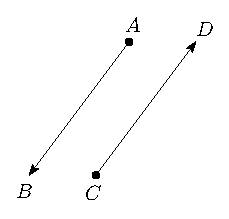
\includegraphics[width=0.2\textwidth]{ANGL4_1.eps}
	\caption{Направленные отрезки $[AB] \neq [CD]$.}
	\label{4_1}
\end{figure}
Следовательно, необходимо что-то для сонаправленности.

\begin{defn}
	Пусть $[AB]$ и $[CD]$ - коллинеарны, не лежат на одной прямой, тогда $[AB]$ и $[CD]$ - \uwave{сонаправлены}, если $B$ и $D$ лежат по одну сторону от прямой $AC$.
\end{defn}
\begin{figure}[H]
	\centering
	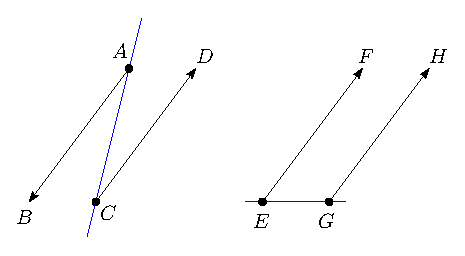
\includegraphics[width=0.4\textwidth]{ANGL4_2.eps}
	\caption{Сонаправленные отрезки $[EF]$ и $[GH]$, и разнонаправленные отрезки $[AB]$ и $[CD]$.}
	\label{4_2}
\end{figure}

\begin{defn}
	Если $[AB]$ и $[CD]$ коллинеарны и лежат на одной прямой, то $[AB]$ и $[CD]$ \uwave{сонаправлены}, если они сонаправлены с направленным отрезком, не лежащим на прямой $AB$.
\end{defn}
\begin{prop}
	Определение выше задано - корректно.
\end{prop}
\begin{proof}
	Пусть $[AB]$ и $[CD]$ сонаправлены с $[EF]$, не лежащим на $AB$. Пусть $[AB]$ и $[GH]$ сонаправлены и $[GH]$ не лежит на одной прямой с $[AB]$, тогда докажем, что $[CD]$ и $[GH]$ сонаправлены. 
	
	$AB$ и $CD$ лежат на одной прямой, $EF ||AB ||GH \Rightarrow CD || GH$. $B$ и $F$ лежат по одну сторону от $AE$. $D$ и $F$ лежат по одну сторону от $EC$. $B$ и $H$ лежат по одну сторону от $AG$. 
	
	Без ограничения общности, поскольку три параллельные прямые можно пересечь одной линией, то передвинем отрезок $[GH]$ вдоль прямой $GH$ до точки пересечения с прямой $AE$. Поскольку и $F$ и $H$ будут по одну сторону с точкой $B$ относительно прямой $AE$, то $[GH]$ и $[EF]$ будут сонаправлены. Аналогичным образом передвинем отрезок $[GH]$ вдоль прямой $GH$ до пересечения с прямой $EC$. 
	\begin{figure}[H]
		\centering
		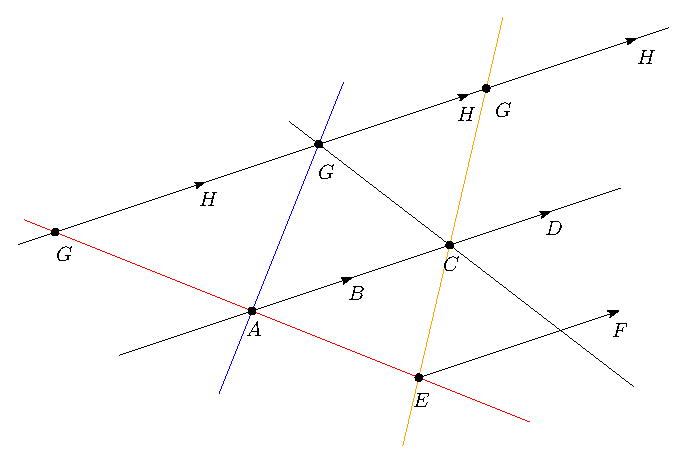
\includegraphics[width=0.55\textwidth]{ANGL4_3.eps}
		\caption{Корректность определения сонаправленности.}
		\label{4_3}
	\end{figure}
	Поскольку точки $D$ и $G$ будут находится по одну сторону от прямой $EC$ и точки $H$ и $F$ также будут находится по одну сторону, то точки $D$ и $H$ также будут находится по одну сторону $\Rightarrow [GH]$ и $[CD]$ будут сонаправленны.
\end{proof}
\begin{defn}
	Отрезки $[AB]\sim [CD]$, если они:
	\begin{enumerate}[label=\arabic*)]
		\item Коллинеарны;
		\item Сонаправлены;
		\item Одинаковой длины;
	\end{enumerate}
\end{defn}
\begin{defn}
	\uwave{Вектор} - это класс эквивалентности относительно $\sim$.
\end{defn}
\begin{defn}
	Класс эквивалентности $[AA]$, называется \uwave{нулевой вектор}, если удовлетворяет ряду свойств:
	\begin{enumerate}[label=\arabic*)]
		\item $[AA]$ коллинеарен любому направленному отрезку;
		\item Сонаправленность не определена;
		\item $[AA] \sim [BB], \, \forall A,B \in \MR^2$;
	\end{enumerate}
\end{defn}

\textbf{\uline{Векторы}}: $\vecm{a} = \vecm{AB}$ - класс эквивалентности $[AB]$, $0$ - нулевой вектор.
\begin{defn}
	Два вектора коллинеарны, если их представители коллинеарны. Нулевой векторо коллинеарен любому вектору.
\end{defn}

\subsection*{Векторы в трехмерном пространстве}
В $\MR^3$ направленные отрезки определяются аналогично и также обозначаются: $[AB]$. Коллинеарность определяется аналогично.
\begin{defn}
	Коллинеарные направленные отрезки $[AB]$ и $[CD]$ \uwave{сонаправлены}, если после их параллельного переноса переводящего $C$ в $A$, образ $D$ и $B$ лежат на прямой $AB$ по одну сторону от $A$.
\end{defn}
\begin{rem}
	Если вектора лежат на одной прямой, то перенесем один из них на параллельную прямую и затем применим это определение.
\end{rem}
\begin{defn}
	Три вектора \uwave{компланарны}, если их представители параллельны одной плоскости.
\end{defn}

\subsection*{Операции с векторами}
Определим операции над векторами.
\begin{enumerate}[label=\arabic*)]
	\item \textbf{Умножение вектора на скаляр}: $\forall \lambda \in \MR$, и для любого вектора $\vecm{a}$, новый вектора $\lambda{\cdot}\vecm{a}$ это:
	\begin{enumerate}[label=(\arabic*)]
		\item Нулевой вектор - $0$, если $\lambda = 0$ или $\vecm{a} = 0$;
		\item Вектор, коллинеарный $\vecm{a}$, длины $|\lambda|{\cdot}|\vecm{a}|$, сонаправленный с $\vecm{a}$, если $\lambda > 0$;
		\item Вектор, коллинеарный $\vecm{a}$, длины $|\lambda|{\cdot}|\vecm{a}|$, направлен в другую сторону с $\vecm{a}$, если $\lambda < 0$;
	\end{enumerate}
	\item \textbf{Сложение векторов}: Пусть $[AB]$ - представитель $\vecm{a}$, $[BC]$ - представитель $\vecm{b}$, тогда $\vecm{a} + \vecm{b}$ определяется, как класс $[AC]$;
	\begin{figure}[H]
		\centering
		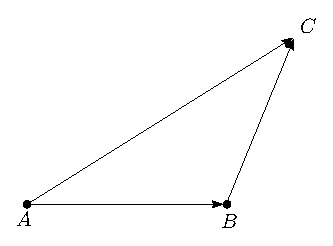
\includegraphics[width=0.25\textwidth]{ANGL4_4.eps}
		\caption{Сложение векторов.}
		\label{4_4}
	\end{figure}
\end{enumerate}
\begin{exrc}
	Проверить независимость от представителя (через параллелограммы).
\end{exrc}
\begin{defn}
	\uwave{Обратным вектором} $-\vecm{a}$ к вектору $\vecm{a}$ называется вектор: $-\vecm{a} \coloneqq (-1){\cdot}\vecm{a}$.
\end{defn}

\textbf{Свойства операций с векторами}
\begin{enumerate}[label=\arabic*)]
	\item \textbf{Коммутативность сложения}: $\vecm{a} + \vecm{b} = \vecm{b} + \vecm{a}$;
	\begin{figure}[H]
		\centering
		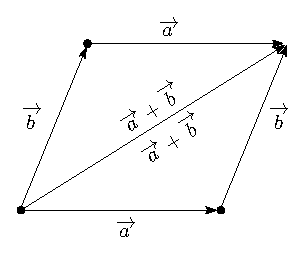
\includegraphics[width=0.25\textwidth]{ANGL4_5.eps}
		\caption{Коммутативность сложения векторов.}
		\label{4_5}
	\end{figure}
	\item \textbf{Ассоциативность сложения}: $\vecm{a} + \left(\vecm{b} + \vecm{c}\right) = \left(\vecm{a} + \vecm{b}\right) + \vecm{c}$;
	\item \textbf{Существование нейтрального элемента по сложению}: $\vecm{a} + \vecm{0} = \vecm{a}$;
	\item \textbf{Существование обратного элемента по сложению}: $\vecm{a} + (-1){\cdot}\vecm{a} = \vecm{0}$;
	\item \textbf{Ассоциативность умножения}: $\forall \alpha,\beta \in \MR, \, (\alpha{\cdot}\beta)\vecm{a} = \alpha{\cdot}(\beta{\cdot}\vecm{a})$;
	\item \textbf{Дистрибутивность относительно сложения}: $\forall \alpha,\beta \in \MR, \, (\alpha + \beta){\cdot}\vecm{a} = \alpha{\cdot}\vecm{a} + \beta{\cdot}\vecm{a}$;
	\item \textbf{Дистрибутивность относительно умножения}: $\forall \alpha \in \MR, \, \alpha{\cdot}\left(\vecm{a} + \vecm{b}\right) = \alpha{\cdot}\vecm{a} + \alpha{\cdot}\vecm{b}$;
	\item \textbf{Существование нейтрального элемента по умножению}: $1{\cdot}\vecm{a} = \vecm{a}$;
\end{enumerate}

\subsection*{Линейная независимость}
Пусть $\vecm{a}_1, \dotsc, \vecm{a}_k$ - векторы.
\begin{defn}
	\uwave{Линейной комбинацией} $\vecm{a}_1, \dotsc, \vecm{a}_k$ называется вектор: $\lambda_1{\cdot}\vecm{a}_1 + \dotsc + \lambda_k{\cdot}\vecm{a}_k, \, \forall i = \overline{1,k}, \, \lambda_i \in \MR$.
\end{defn}

\begin{defn}
	Линейная комбинация называется \uwave{тривиальной}, если $\lambda_1 = \lambda_2 = \dotsc = \lambda_n = 0$ и \uwave{нетрививальной} в противном случае.
\end{defn}

\begin{defn}
	Вектора $\vecm{a}_1, \dotsc, \vecm{a}_k$ называются \uwave{линейно зависимыми}, если существует хотя бы одна их нетривиальная линейная комбинация равная $0$.
\end{defn}

\begin{defn}
		Вектора $\vecm{a}_1, \dotsc, \vecm{a}_k$ называются \uwave{линейно независимыми}, если любая их линейная комбинация, равная нулю, является тривиальной.
\end{defn}
Ещё это можно сформулировать по-другому:
\begin{enumerate}[label=\arabic*)]
	\item $\vecm{a}_1, \dotsc, \vecm{a}_k$ - \uwave{линейно зависимы} $\Leftrightarrow \exists\, \lambda_1,\dotsc,\lambda_k$ не все равные $0 \colon \lambda_1{\cdot}\vecm{a}_1 + \dotsc + \lambda_k{\cdot}\vecm{a}_k = 0$;
	\item $\vecm{a}_1, \dotsc, \vecm{a}_k$ - \uwave{линейно независимы} $\Leftrightarrow  \lambda_1{\cdot}\vecm{a}_1 + \dotsc + \lambda_k{\cdot}\vecm{a}_k = 0 \Rightarrow \lambda_1 = \dotsc = \lambda_k = 0$;
\end{enumerate}

\begin{prop}
	Вектора $\vecm{a}$ и $\vecm{b}$ - линейно зависимы $\Leftrightarrow \vecm{a}$ и $\vecm{b}$ - коллинеарны.
\end{prop}
\begin{proof}\hfill\\
	$(\Rightarrow)$ Пусть $\vecm{a}$ и $\vecm{b}$ - линейно зависимы $\Rightarrow \lambda_1 \neq 0 \vee \lambda_2 \neq 0 \colon \lambda_1\vecm{a} + \lambda_2 \vecm{b} = 0$. Пусть $\lambda_1 \neq 0$, тогда: 
	$$
		\lambda_1 \neq 0, \, \lambda_1 \vecm{a} + \lambda_2 \vecm{b} = 0 \Rightarrow \vecm{a} + \dfrac{\lambda_2}{\lambda_1}\vecm{b} = 0 \Rightarrow \vecm{a} = -\dfrac{\lambda_2}{\lambda_1}\vecm{b}
	$$
	то есть $\vecm{a}$ и $\vecm{b}$ - коллинеарны.
	
	$(\Leftarrow)$ Пусть $\vecm{a}$ и $\vecm{b}$ - коллинеарны $\Rightarrow$ возможно несколько ситуаций:
	\begin{enumerate}[label=\arabic*)]
		\item $\vecm{a} = \vecm{b} = \vecm{0} \Rightarrow 1{\cdot}\vecm{a} + 0{\cdot}\vecm{b} = \vecm{0} \Rightarrow$ линейно зависимы;
		\item $\vecm{a}  = 0, \vecm{b}  \neq 0 \Rightarrow 1{\cdot}\vecm{a} + 0{\cdot}\vecm{b} = 0 \Rightarrow$ линейно зависимы; 
		\item $\vecm{a}  \neq 0, \vecm{b} = 0 \Rightarrow 0{\cdot}\vecm{a} + 1{\cdot}\vecm{b} = 0 \Rightarrow$ линейно зависимы;
		\item $\vecm{a}  \neq 0, \vecm{b} \neq 0 \Rightarrow \vecm{a} = \dfrac{\big| \vecm{a}\big|}{\big| \vecm{b}\big|}\vecm{b}$, если сонаправленны и $\vecm{a} = -\dfrac{\big| \vecm{a}\big|}{\big| \vecm{b}\big|}\vecm{b}$ иначе, тогда $\big|\vecm{b}\big|{\cdot}\vecm{a} \pm \big|\vecm{a}\big|{\cdot}\vecm{b} \Rightarrow$ линейно зависимы;
	\end{enumerate}
\end{proof}

\begin{prop}
	Вектора $\vecm{a}, \vecm{b}$ и $\vecm{c}$ - линейно зависимы $\Leftrightarrow \vecm{a}, \vecm{b}$ и $\vecm{c}$ - компланарны.
\end{prop}
\end{document}